% Copyright © 2015 Martin Ueding <dev@martin-ueding.de>
%
\documentclass[english, fleqn]{beamer}

%\usetheme{default}
\useoutertheme{infolines}

\usecolortheme{whale}
%\usecolortheme{rose}

\usepackage[beamer]{header}

\renewcommand\iup{\text i}
\renewcommand\eup{\text e}

\title{Analysis of $\piup$--$\piup$ scattering data}
%\subtitle{}
\author{Martin Ueding – mu@martin-ueding.de}
\date{2015-03-20}

\AtBeginSection[]
{
    \begin{frame}
        \sectionpage
        \tableofcontents[sectionstyle=show/shaded, subsectionstyle=show/shaded/hide]
    \end{frame}
}

\AtBeginSubsection[]
{
    \begin{frame}
        \subsectionpage
        \tableofcontents[sectionstyle=show/shaded, subsectionstyle=show/shaded/hide]
    \end{frame}
}

\begin{document}

\nocite{Knippschild/Pi_Pi_Scattering}

\begin{frame}
    \titlepage
\end{frame}

\begin{frame}
    \frametitle{Contents of this presentation}
    \tableofcontents
\end{frame}

\section{Data generation}

\subsection{Metropolis algorithm}

\subsection{Correlation functions}


\section{Analysis}

\newcommand\scale{0.2}

\subsection{Importing data}

\begin{frame}
    \frametitle{Input data}
    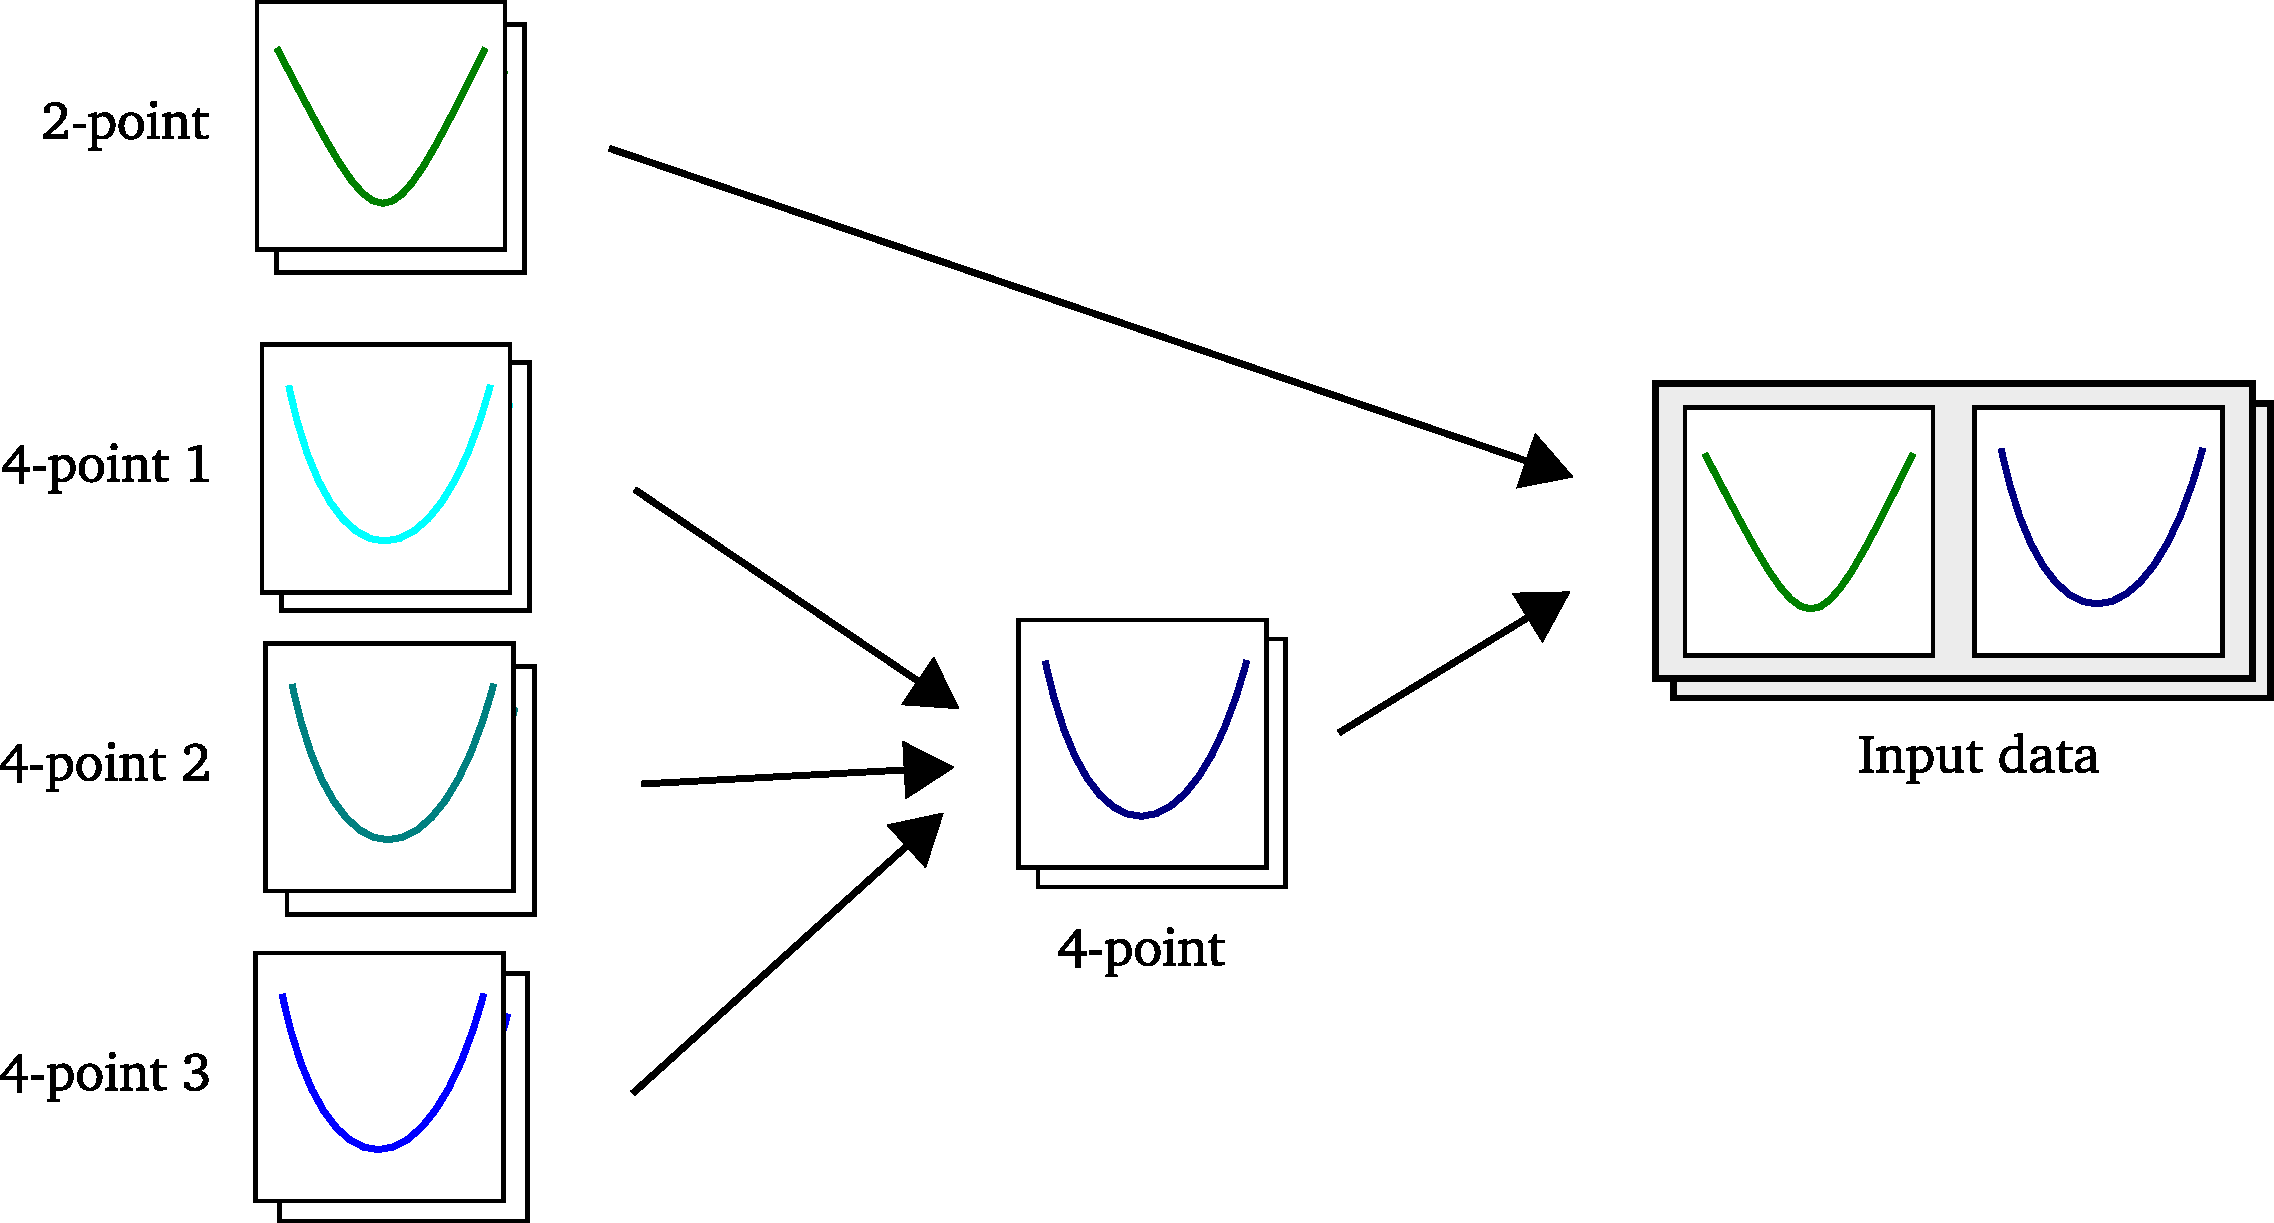
\includegraphics[scale=\scale]{sketches/01-input.pdf}
\end{frame}

\begin{frame}
    \frametitle{Folding}
    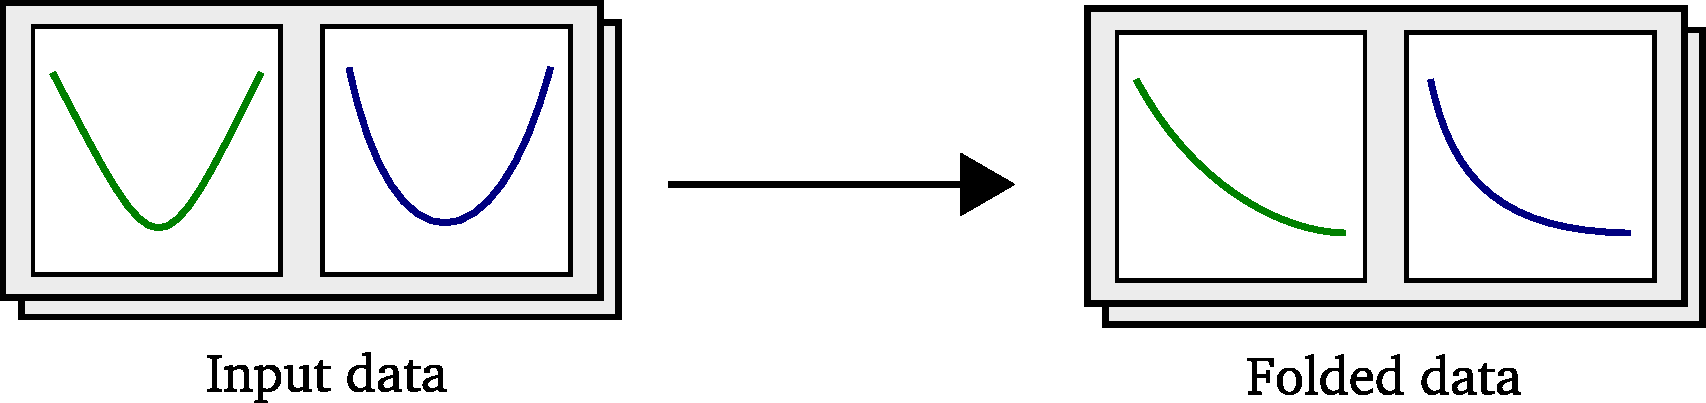
\includegraphics[scale=\scale]{sketches/02-folding.pdf}
\end{frame}

\subsection{Bootstrap}

\begin{frame}
    \frametitle{Bootstrap}
    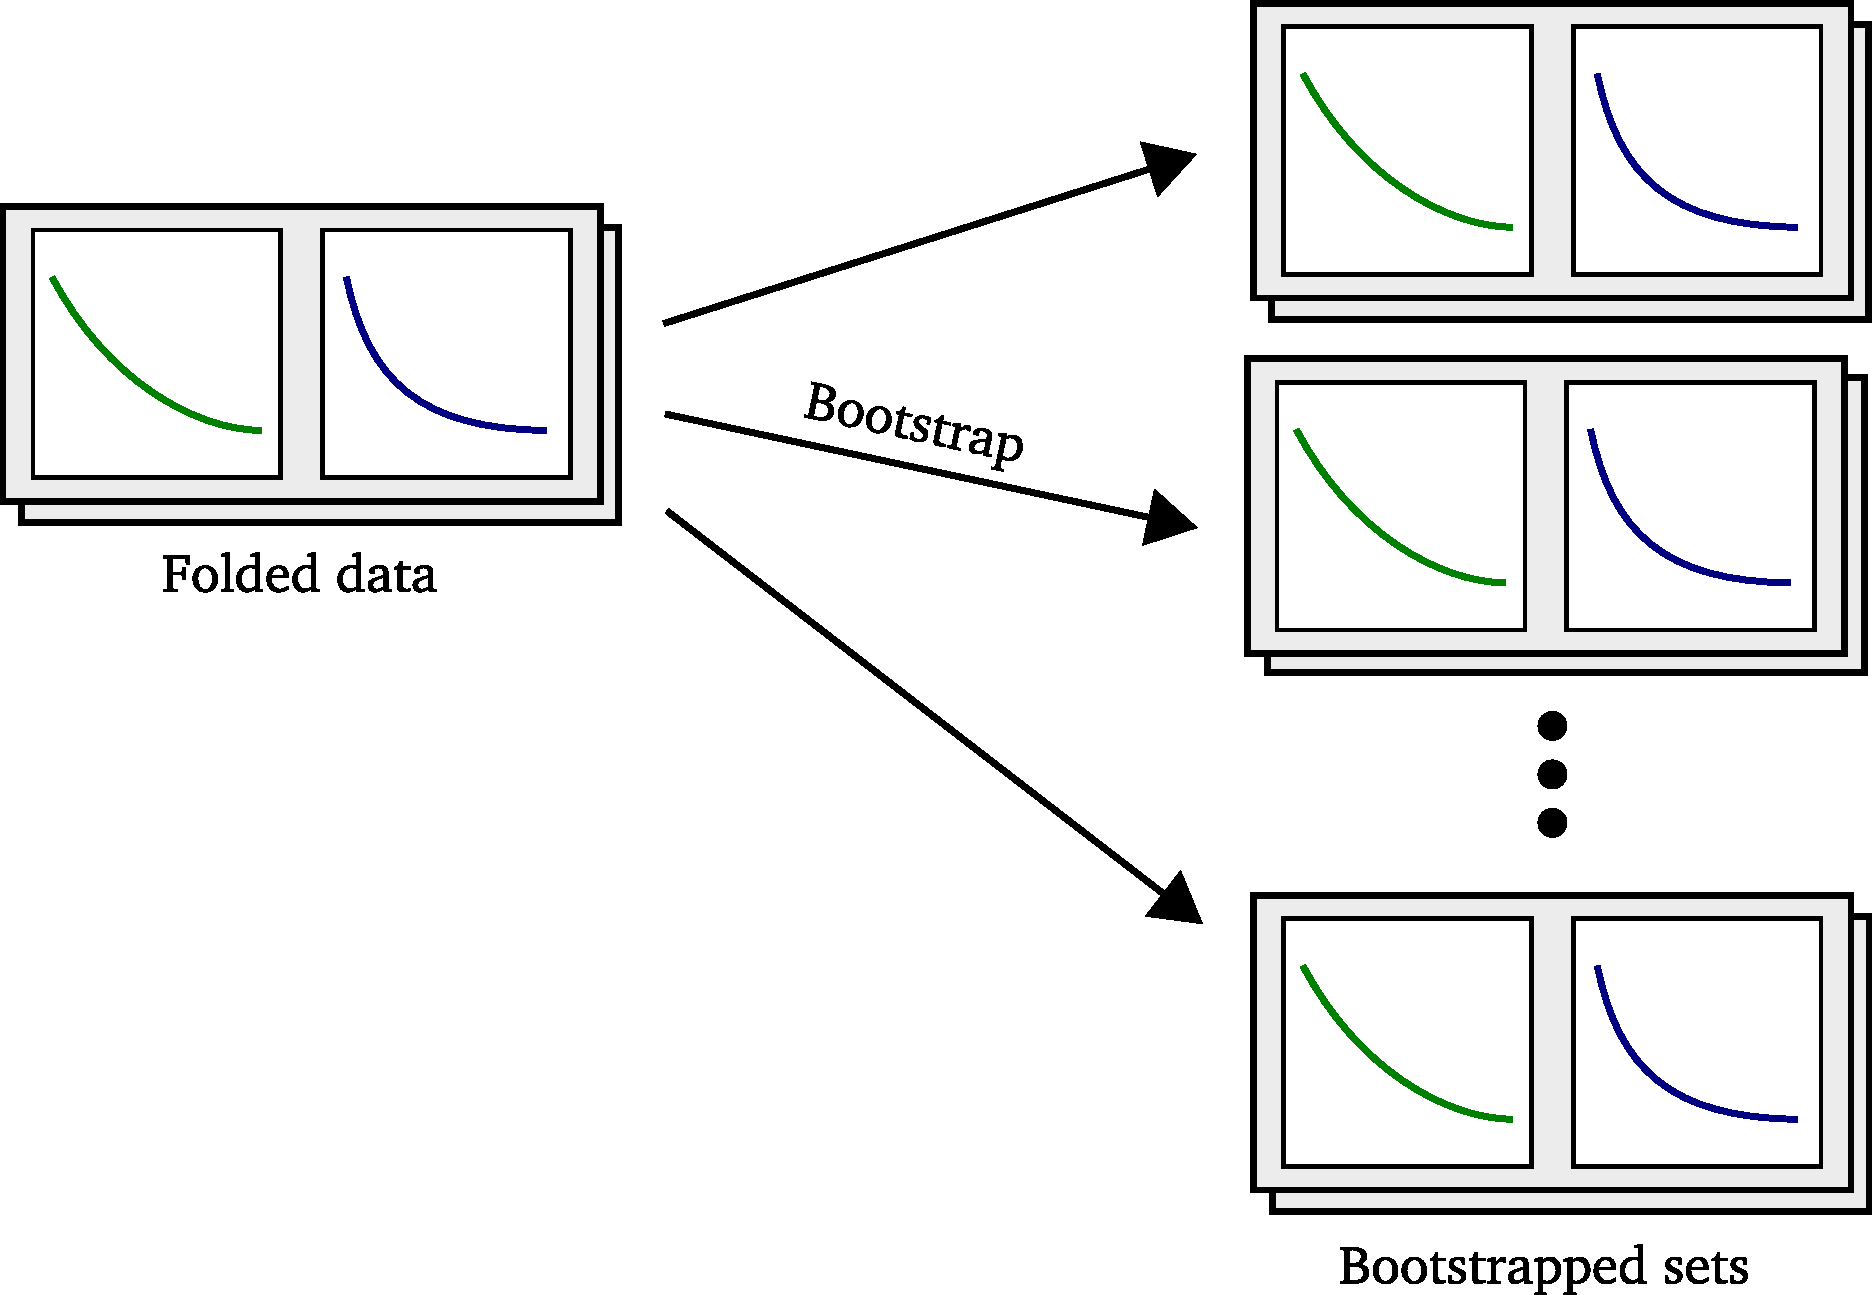
\includegraphics[scale=\scale]{sketches/03-bootstrap.pdf}
\end{frame}

\begin{frame}
    \frametitle{Bootstrap}
    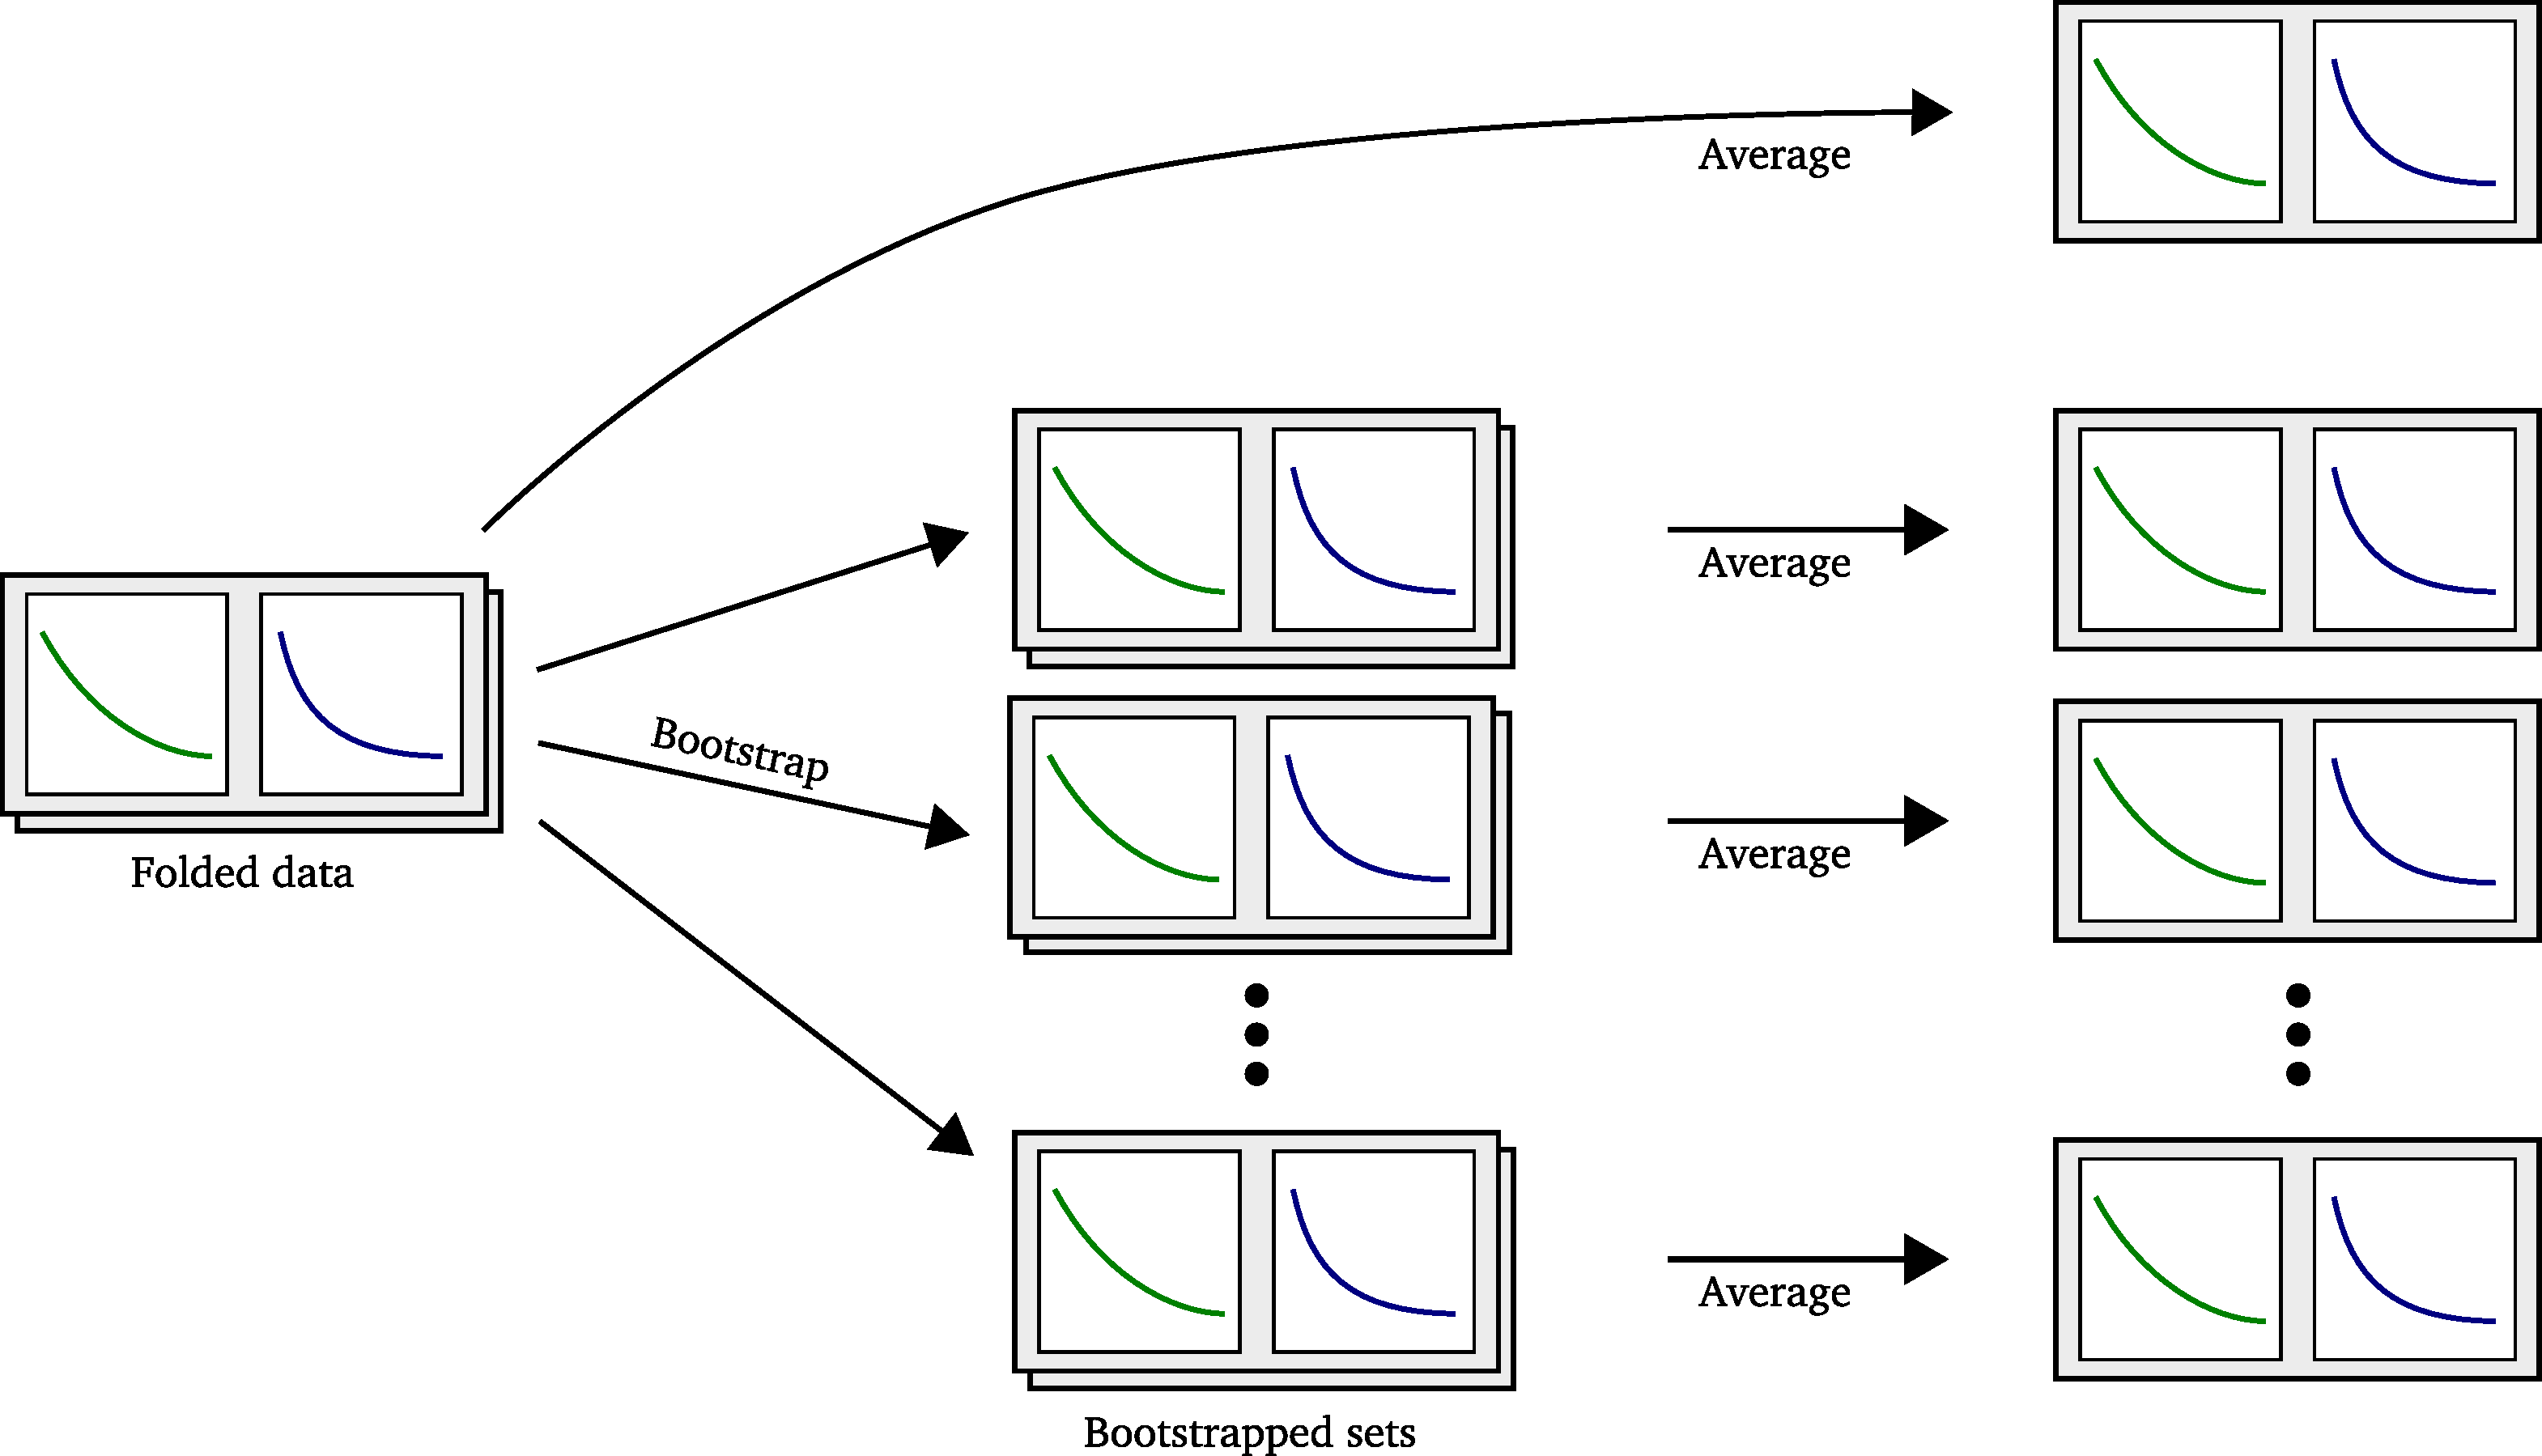
\includegraphics[scale=\scale]{sketches/04-bootstrap.pdf}
\end{frame}

\subsection{Correlated fit}

\begin{frame}
    \frametitle{Correlation matrix}
    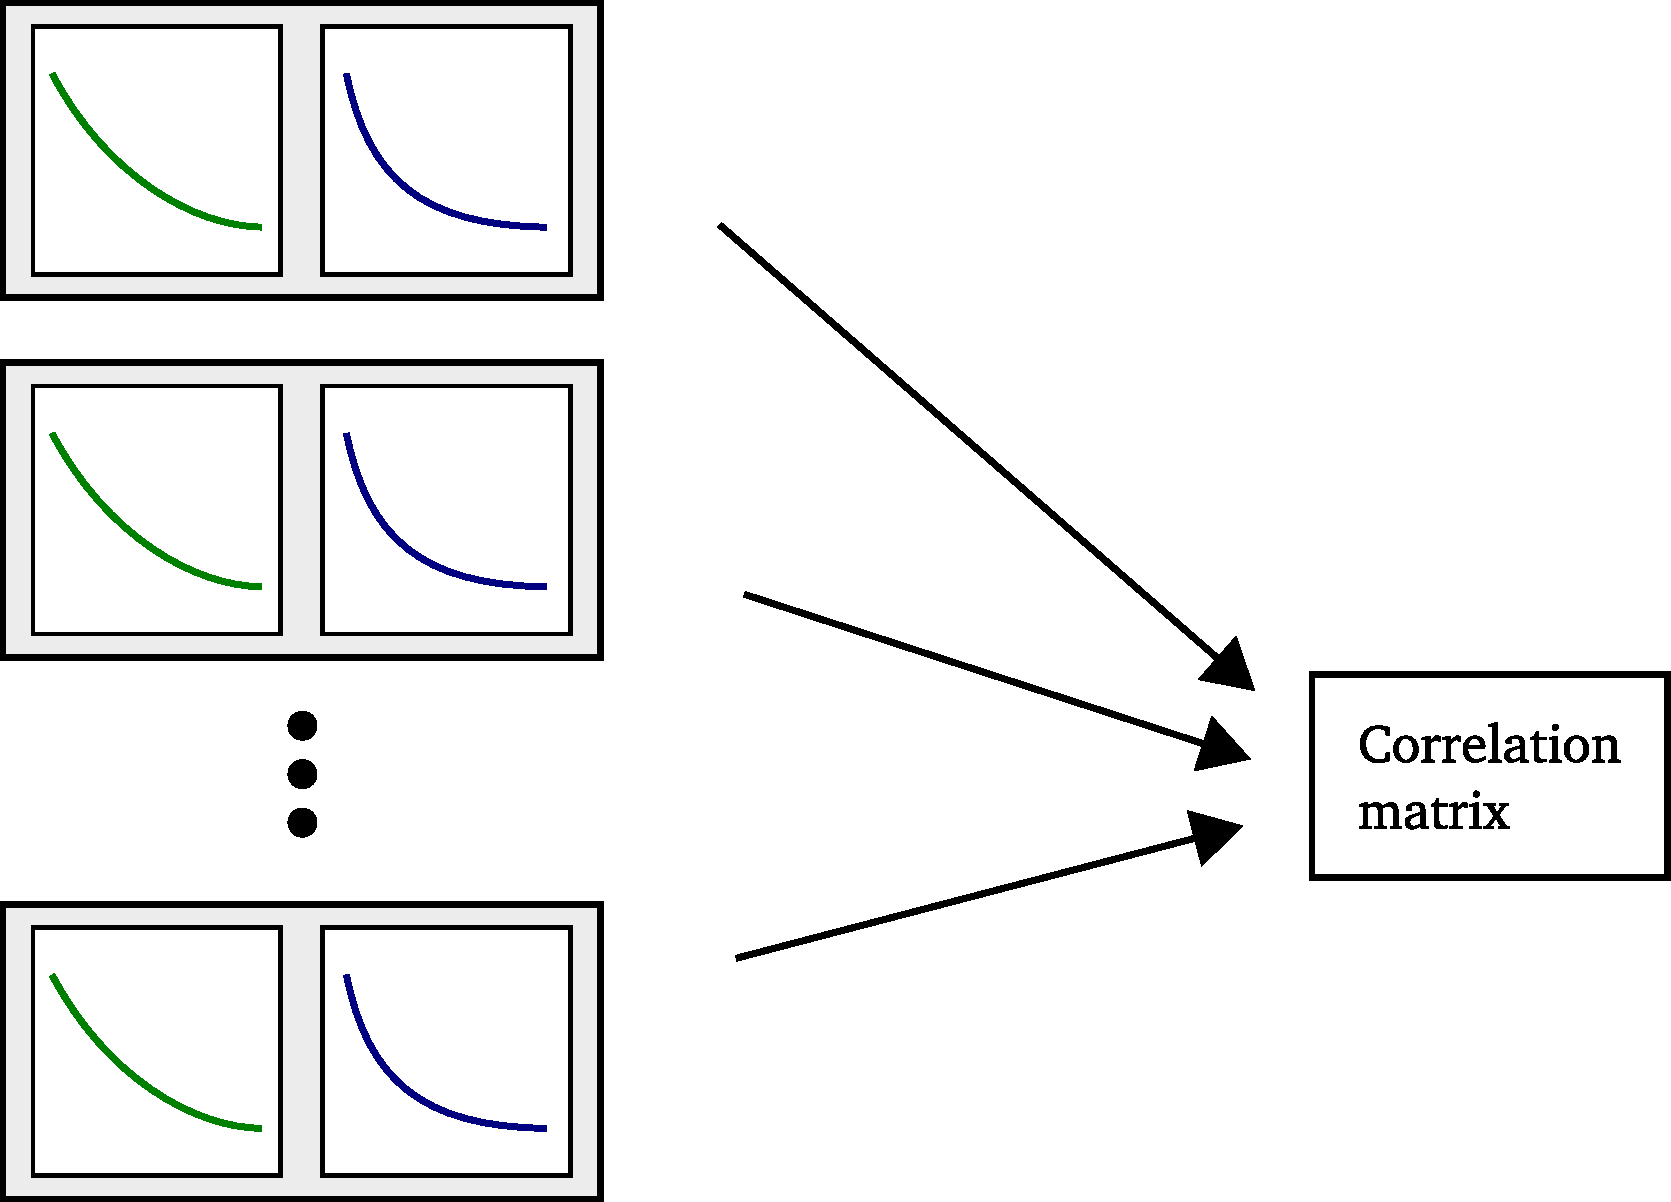
\includegraphics[scale=\scale]{sketches/05-matrix.pdf}
\end{frame}

\begin{frame}
    \frametitle{Correlated fit}
    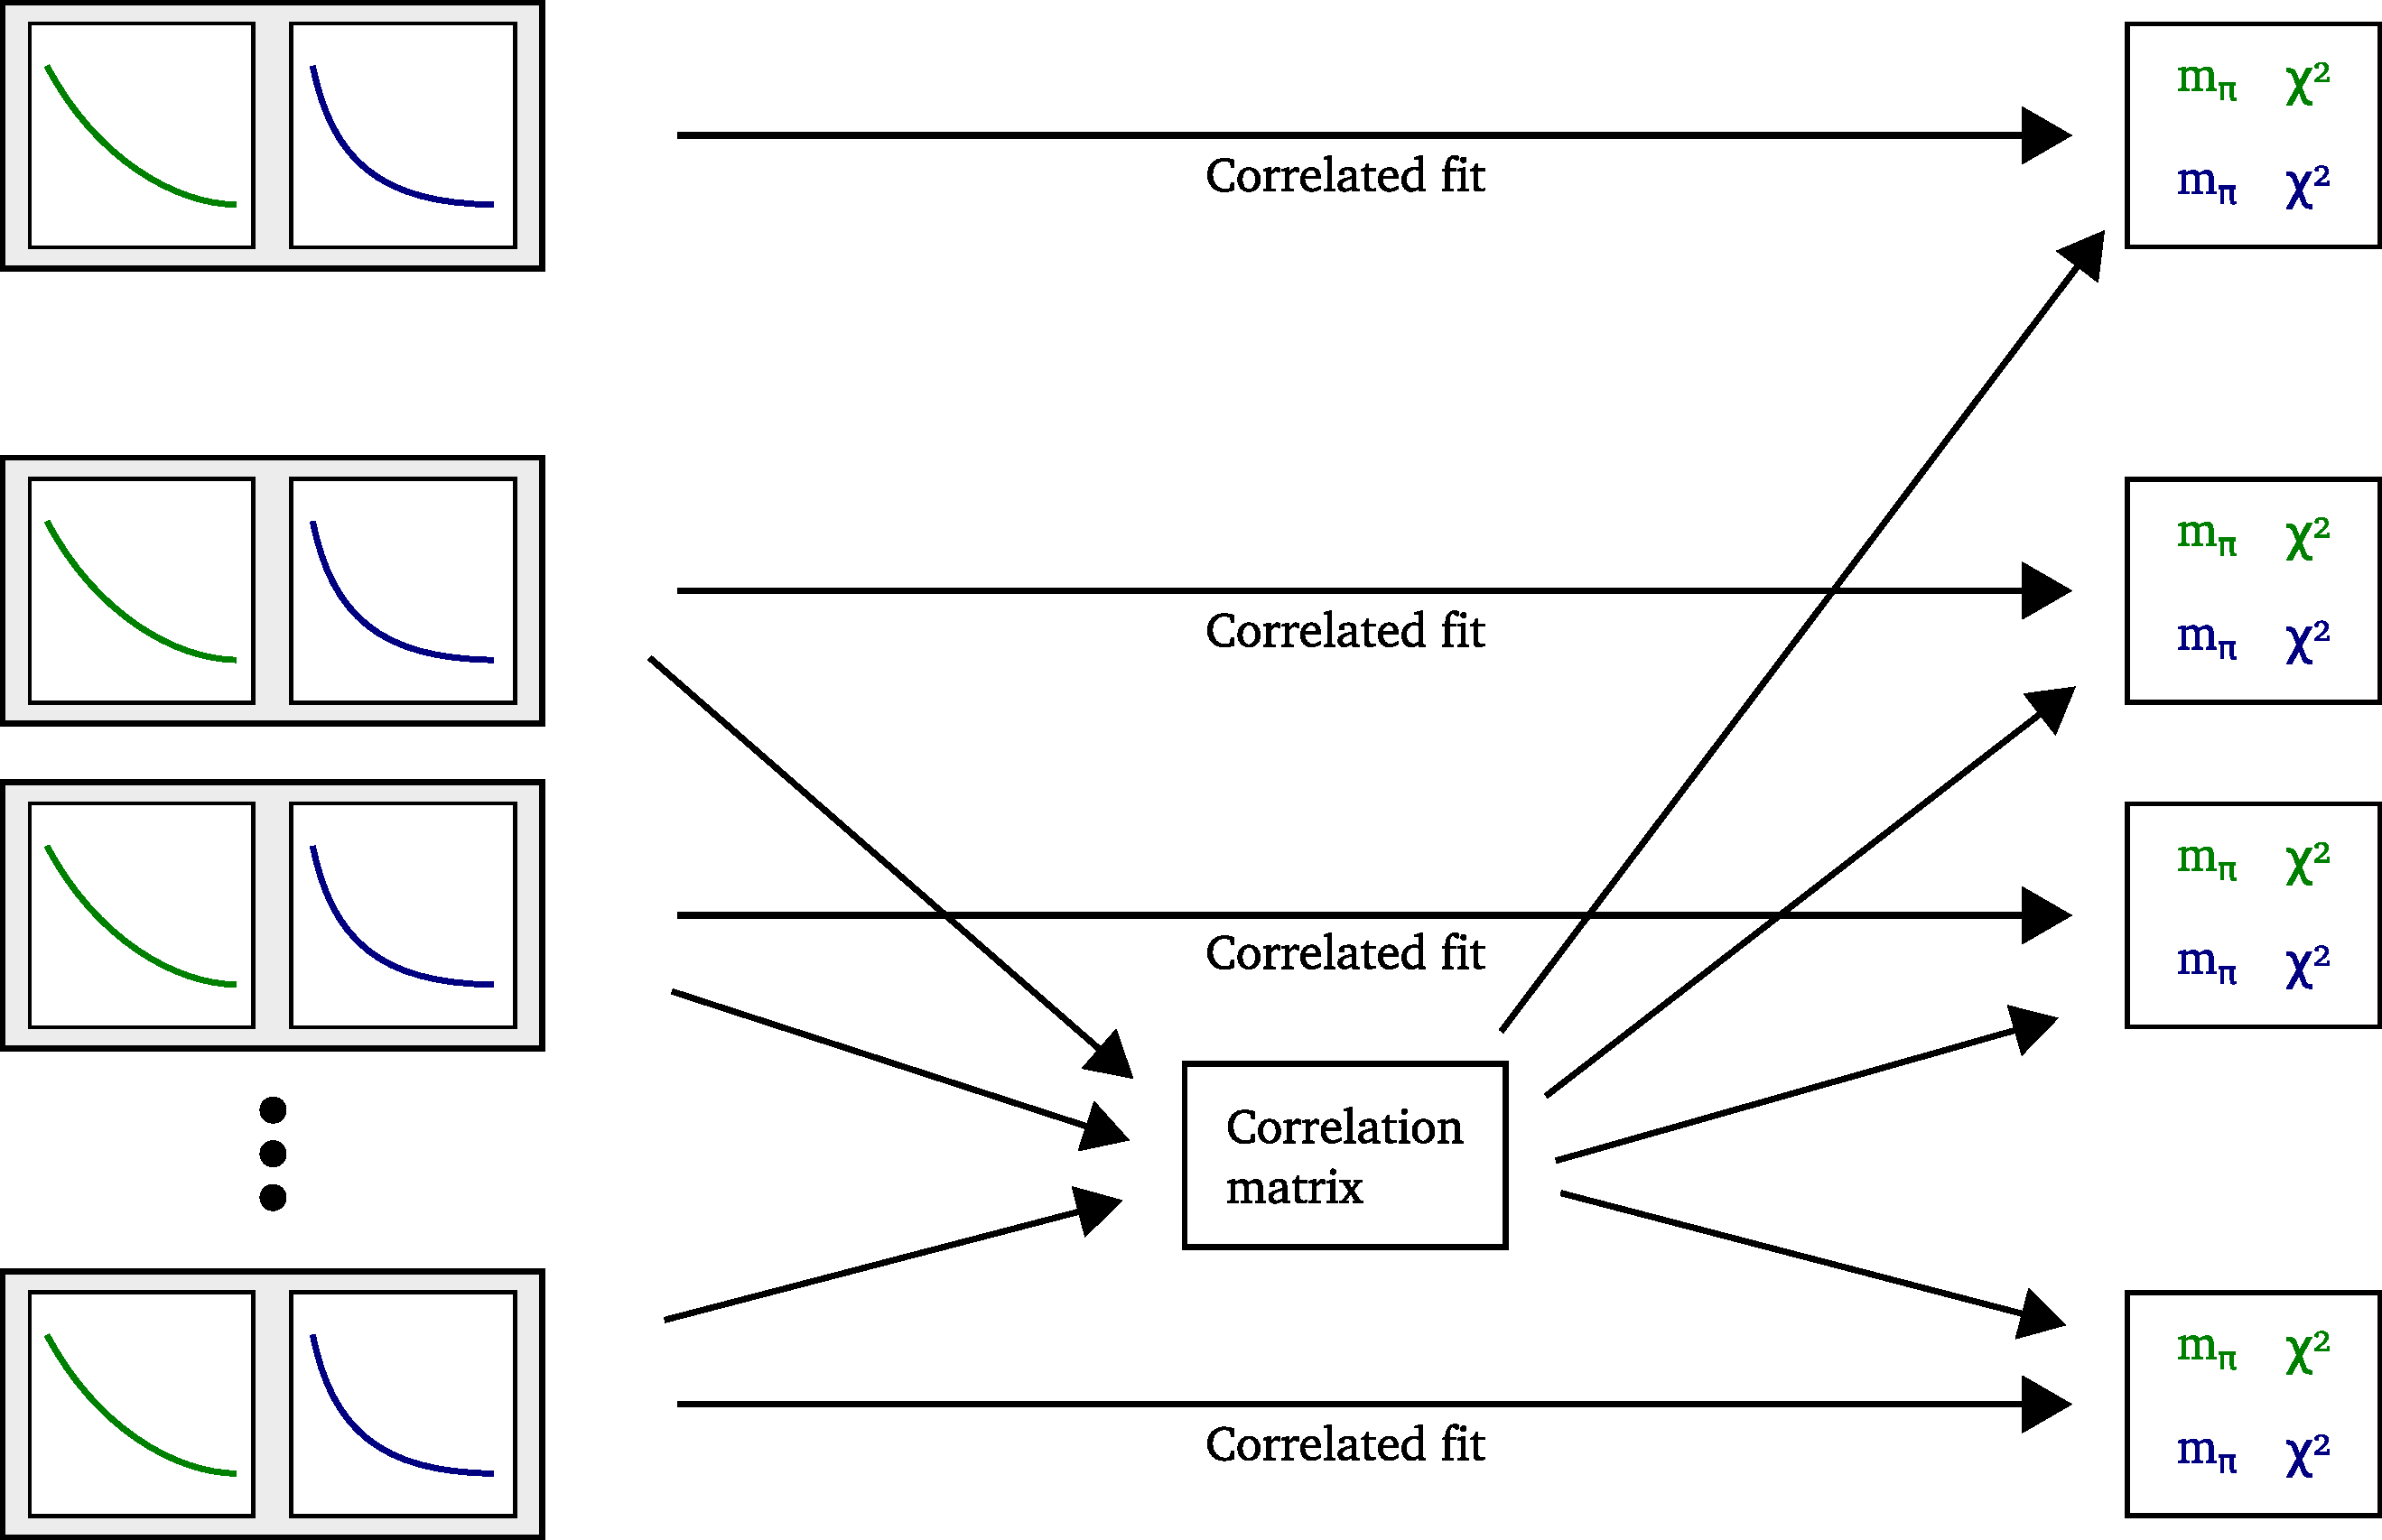
\includegraphics[scale=\scale]{sketches/06-fit.pdf}
\end{frame}

\subsection{Scattering length}

\begin{frame}
    \frametitle{Lüscher formula}
    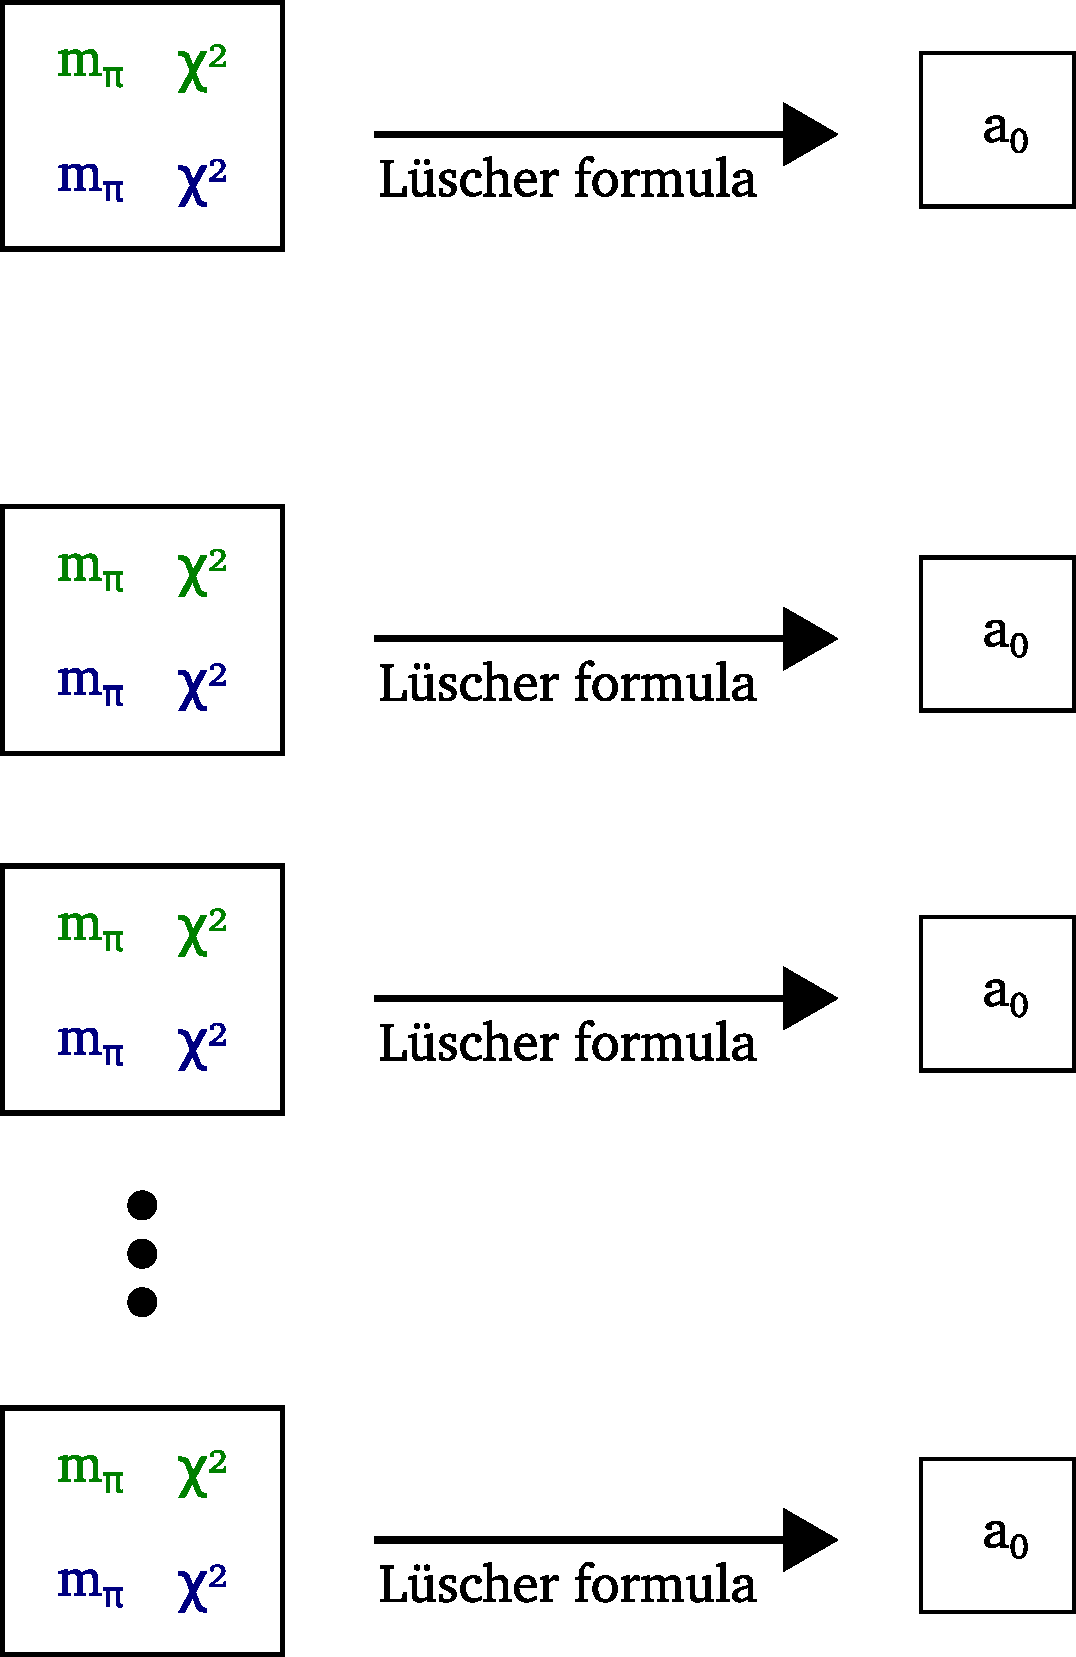
\includegraphics[scale=\scale]{sketches/07-luescher.pdf}
\end{frame}

\begin{frame}
    \frametitle{End results}
    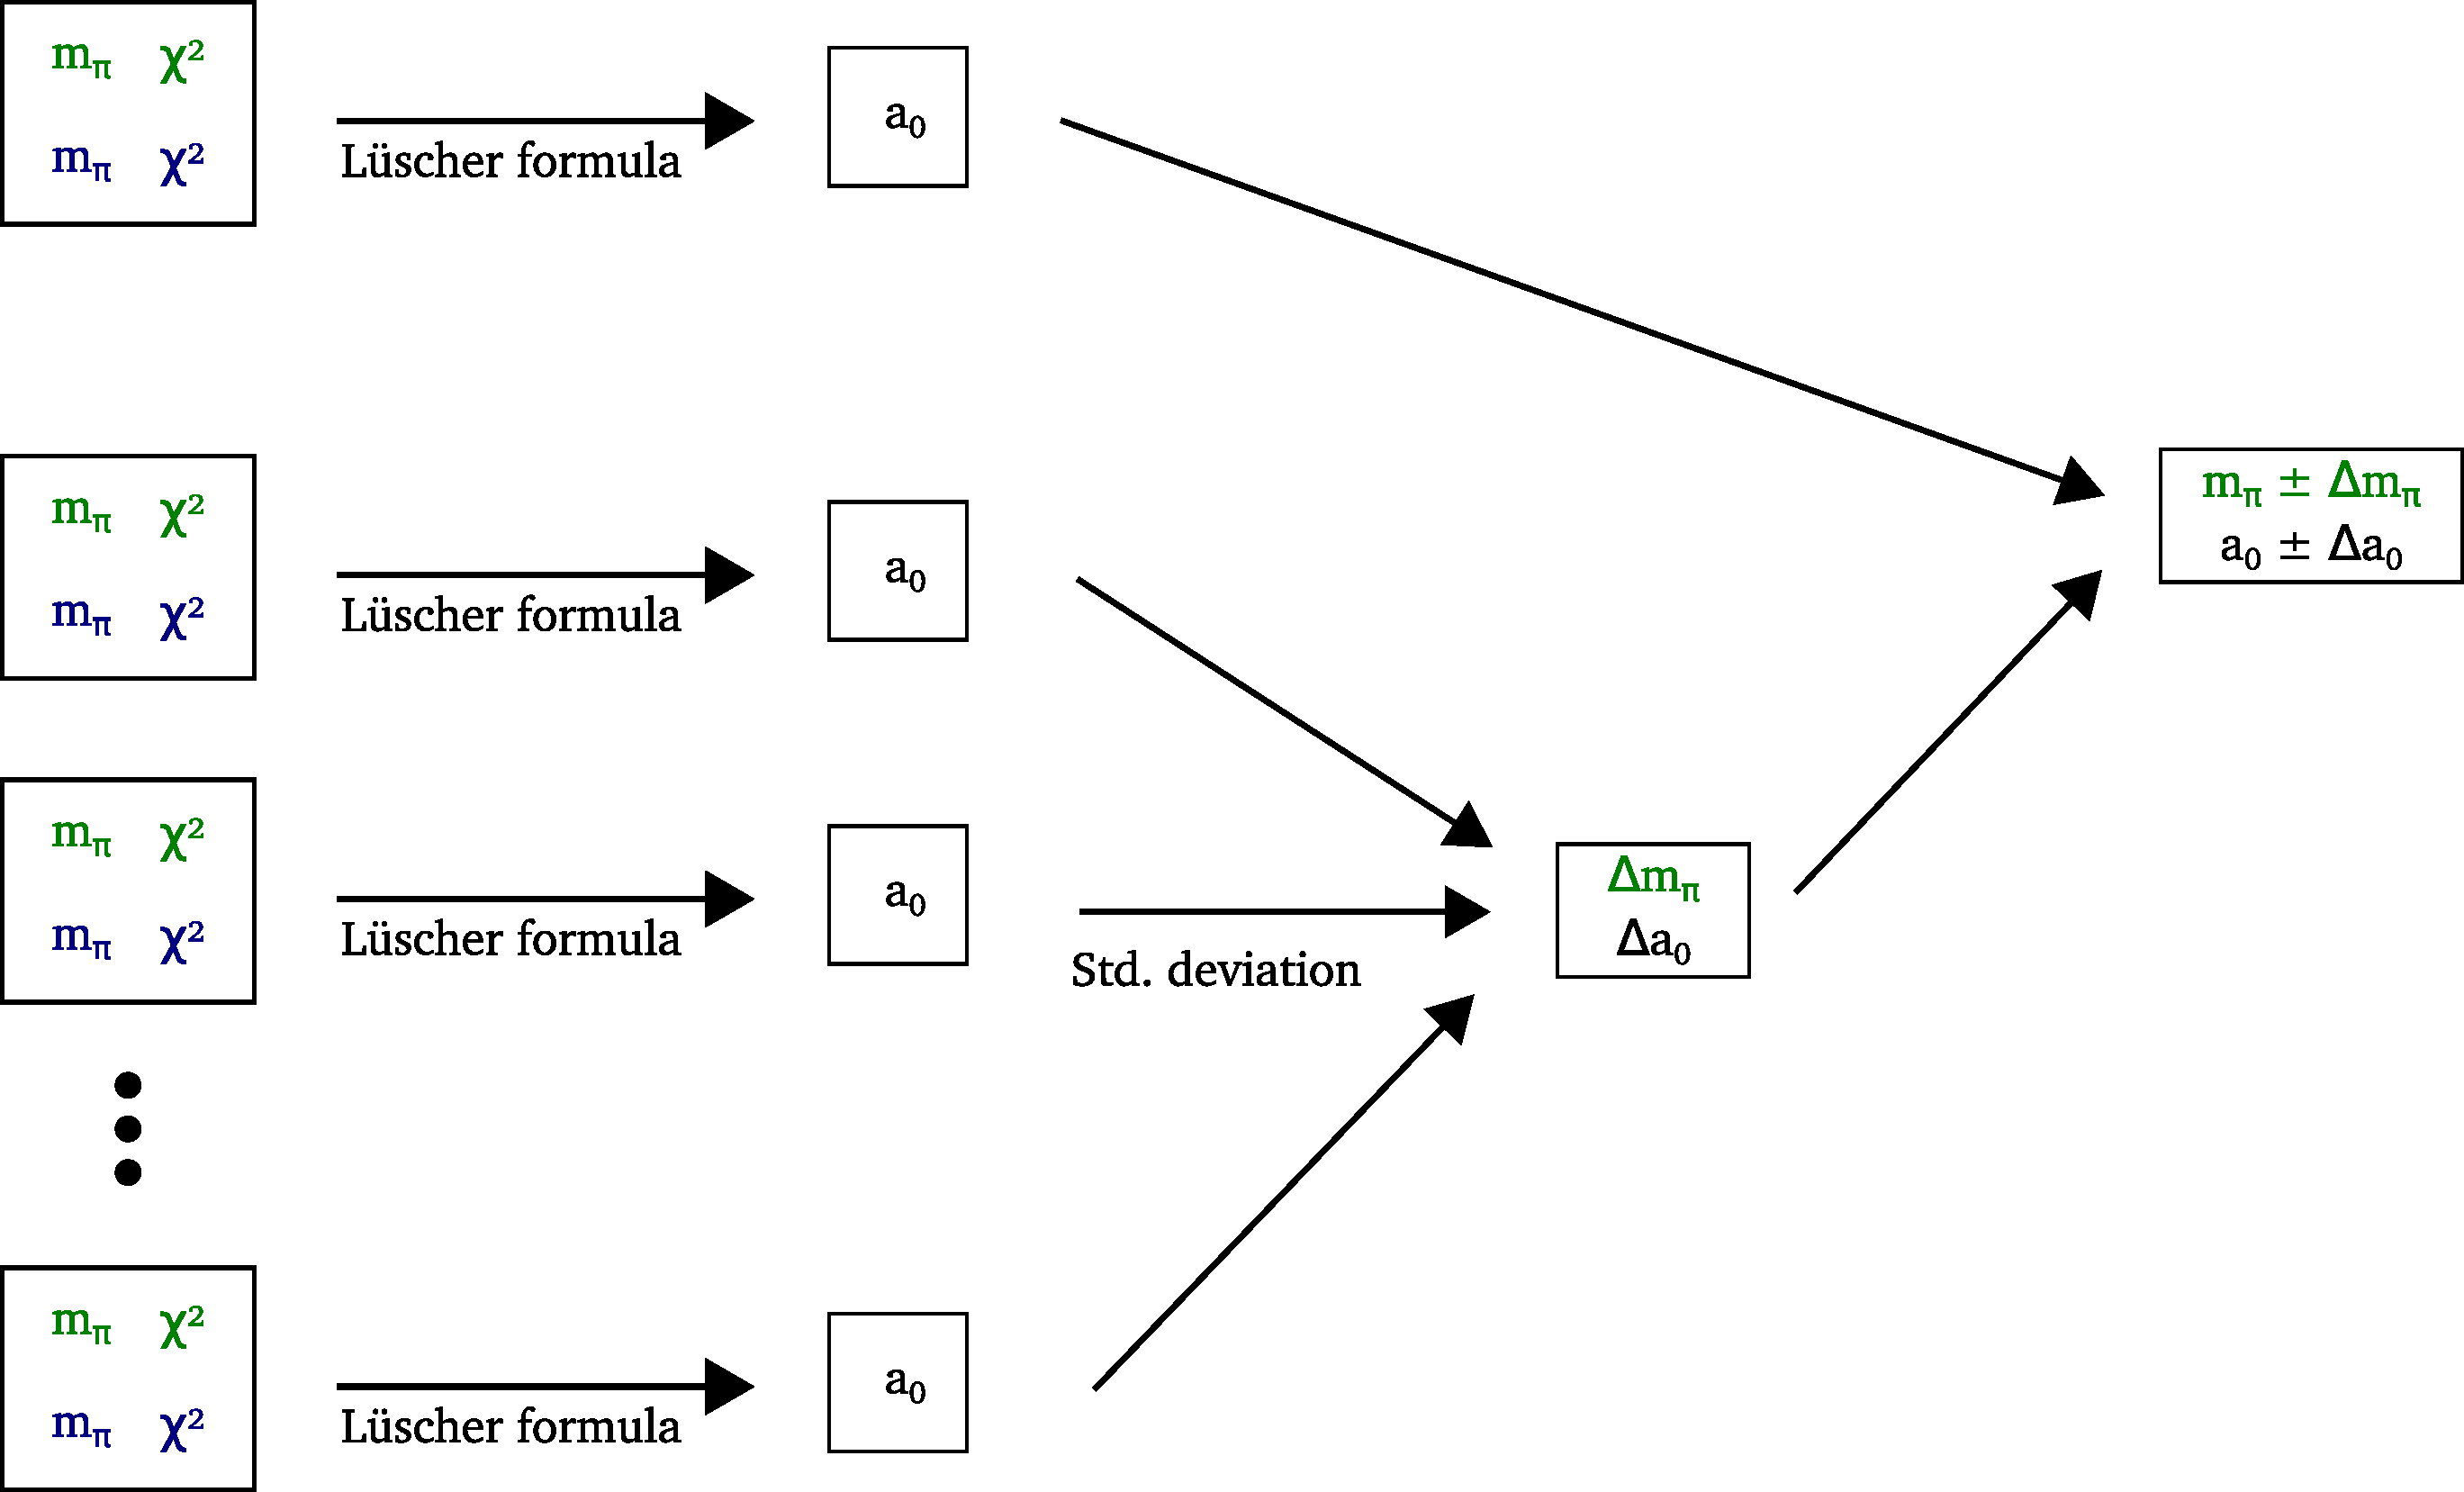
\includegraphics[scale=\scale]{sketches/08-end-result.pdf}
\end{frame}

%\section{References}

\begin{frame}
    %\frametitle{References}

    \printbibliography
\end{frame}

\end{document}

% vim: spell spelllang=en
